\chapter{ARMA}
\label{ARMA}
The Autoregressive Moving Average Model(ARMA) combines both the AR and MA models. The Autoregressive component involves regressing the variable based on its own previous values. The Moving Average component models the error term as a linear combination of both current and past error terms.

The ARMA model of order $(p,q)$ can be formulated as:
\begin{equation}
    y_{t}=\mu_{0}+\epsilon_t +\sum^{p}_{i=1}\alpha_{i} y_{t-i} + \sum^{q}_{j=1}\theta{j} \epsilon_{t-j}
\end{equation}
where $\mu_{0}$ is the mean of the timeserie, $\epsilon_{t}, \epsilon_{t-1}, ..., \epsilon_{t-q}$ are the error terms, $\alpha_{i}$ and $\theta_{j}$ are the parameters of the model, and $y_{t-1}, y_{t-2}, ..., y_{t-p}$ are the past values.

For our purpose we decided to implement only the ARMA(1,1) model, which can be rewritten in the following way:
\begin{equation}
    \label{ARMA_q1}
    y_{t}=\mu_{0}+\epsilon_t +\alpha y_{t-1} + \theta \epsilon_{t-1} \qquad 
    \epsilon_t \stackrel{iid}{\sim} \mathcal{N}(0,\sigma^2)
\end{equation}
and again we assume $\epsilon_{t}$ to be independent and identical distributed variables coming from a normal distribution with mean $0$ and variance $\sigma^2$.

\section*{ARMA(1,1)}
Given the equation \refeq{ARMA_q1} the likelihood of the ARMA model can be expressed as:
\begin{equation}
    y_{t}|\mu_{0},\alpha,\theta,\sigma^2,y_{t-1},\epsilon_{t-1}\sim \mathcal{N}(\mu_{0} + \alpha y_{t-1} + \theta \epsilon_{t-1}, \sigma^2)
\end{equation}
and we selected the following priors:
\begin{equation}
    \begin{split}
        \mu_0 \sim \mathcal{N}(0.0, 10000) \\
        \tau = 1 / \sigma^2 \sim \mathcal{G}(2, 0.1) \\
        \alpha \sim \mathcal{U}(-1.0, 1.0) \\
        \theta \sim \mathcal{U}(-1.0, 1.0)
    \end{split}
\end{equation}
such that $\mu_{0}$ and $\sigma^2$ have uninformative distributions, while $\alpha$ adheres to the stationary constraint for the AR part.

We produced the traceplots and autocorrelation plots to verify the validity of our assumptions and we obtained the following posteriors for the parameters: \\
\begin{figure}[h]
    \centering
    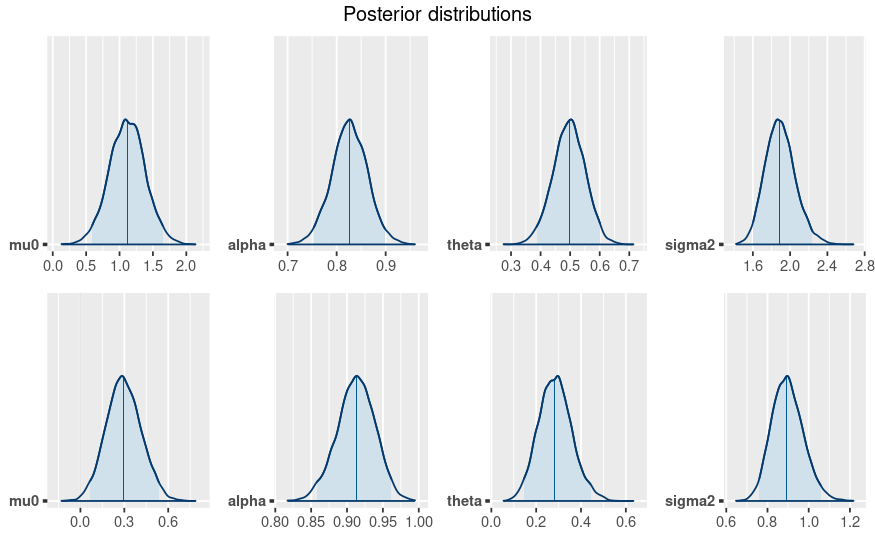
\includegraphics[width=\textwidth]{../Images/4-ARMA/posteriors.png}
    \caption{The image displays the posterior distributions of the parameters for the ARMA(1,1) model. The top line corresponds to the model used for GDP, while the bottom line corresponds to the model used for inflation.}
    \label{fig:ARMA_posteriors}
\end{figure} \\

Finally we plotted the in-sample and out-of-sample predictions with credible intervals and we compared it with the true data: \\    
\begin{figure}[h]
    \centering
    \begin{minipage}[t]{0.7\textwidth}
        \centering
        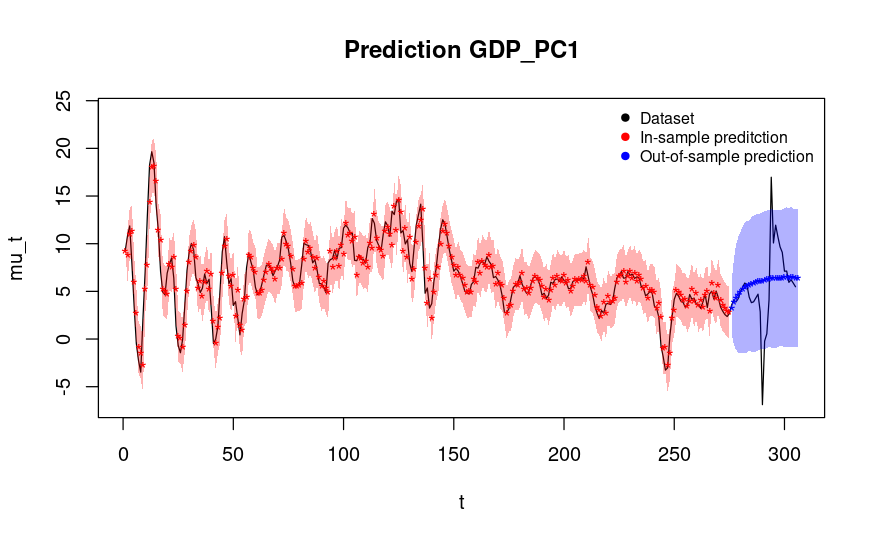
\includegraphics[width=\textwidth]{../Images/4-ARMA/gdp_prediction.png}
        \label{fig:ARMA_first}
    \end{minipage}
    \begin{minipage}[t]{0.7\textwidth}
        \centering
        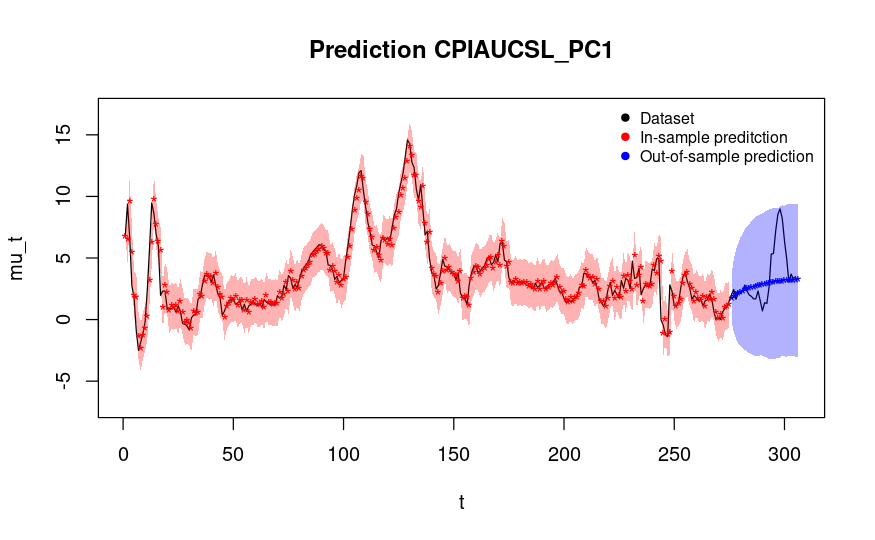
\includegraphics[width=\textwidth]{../Images/4-ARMA/infl_prediction.png}
        \label{fig:ARMA_second}
    \end{minipage}
    \caption{ARMA(1,1): In-sample and out-of-sample predictions}
    \label{fig:ARMA_combined}
\end{figure} \\
In the Appendix it is possible to find a comparison between our model the ARIMA function used to verify the model's correctness.